%\documentclass[twoside,a4paper]{report}
\documentclass[a4paper, twocolumn]{article}

\usepackage[utf8]{inputenc}

\usepackage{hyperref}
\usepackage{graphicx}
\usepackage{tabularx}
\usepackage{supertabular}
\usepackage{pdflscape} %% Used for very big table
\usepackage{moreverb}
\usepackage[table]{xcolor}
\usepackage{listings}
\usepackage{paralist}
\usepackage{fancyhdr}
\usepackage[draft]{fixme}
\fxsetup{footnote}
\fxsetup{nomargin}

\definecolor{codegray}{gray}{.95}
\definecolor{palegray}{gray}{.65}
\lstset{language=C,
	numbers=left,
	tabsize=2,
	basicstyle=\scriptsize,
	stringstyle=\textrm,
	showstringspaces=false,
	frame=none,
	xleftmargin=3pt,
	backgroundcolor=\color{codegray}}

\title{Current State of Knowledge Representation Systems for Robotics}
\author{Séverin Lemaignan, Moritz Tenorth}

\graphicspath{{figs/}}

\newcommand{\ie}{{\textit{i.e.~}}}
\newcommand{\cf}{{\textit{cf~}}}
\newcommand{\eg}{{\textit{e.g.~}}}

\begin{document}

\maketitle
\tableofcontents

%%%%%%%%%%%%%%%%%%%%%%%%%%%%%%%%%%%%%%%%%%%%%%%%%%%%%%%%%%%%%%%%%%%%%%%%%%%%%%%%%%%%%%%%%%%
\section{Introduction}
\label{sect|intro}

The idea of \emph{Cognitive Robotics} was coined in the early 1990s by Reiter.
In a chapter on that subject in \emph{Fondations of Artifical
Intelligence}~\cite{Levesque2008}, Levesque reminds about the manifesto they
wrote together in 1998:

\begin{quotation}

	Central to this effort is to develop an understanding of the relationship
	between the knowledge, the perception, and the action of such a robot. The
	sorts of questions we want to be able to answer are

	\begin{itemize} 
	
		\item to execute a program, what information does a robot need to have
		at the outset vs. the information that it can acquire \emph{en route}
		by perceptual means?

		\item what does the robot need to know about its environment vs. what
		need only be known by the designer?

		\item when should a robot use perception to find out if something is
		true as opposed to reasoning about what it knows was true in the past?

		\item when should the inner workings of an action be available to the
		robot for reasoning and when should the action be considered primitive
		or atomic?

	\end{itemize}

	and so on. With respect to robotics, our goal (like that of many in AI) is
	\emph{high-level robotic control}: develop a system that is capable of
	generating actions in the world that are appropriate as a function of some
	current set of beliefs and desires.

\end{quotation}

This survey focuses on the knowledge issue: we aims at establishing the current
landscape of approaches to the knowledge representation problem in the research
community, at summarizing the major trends and identifying the possible
shortcomings.

We have identified over ten projects that either are explicitely advertised as
knowledge representation systems or involve explicit knowledge manipulation
within a robot. By knowledge manipulation, we mean symbolic representation of
assertions, be it static statements on the world or spatio-temporal events, and
reasoning on this representation.

We also try, for each project, to make clear \begin{inparaenum} \item how new
facts can be acquired, \ie how informations from perception or interaction are
turned into knowledge, \item how, in return, symbolic concept are
\emph{anchored} into the robot sensori-motor space, \item how the knowledge
representation system integrates with the decisional layers of the robot, and
how this leads to better robotic control.\end{inparaenum}


\subsection{Definition of inclusion criteria}
\label{sect|inclusion-criteria}

Every robotic system has, implicitely or not, some knowledge representation
systems. It may range from a simple state vector to an explicit symbolic
knowledge base.  This survey focuses on the right end of this spectrum:
symbolic systems, suited for abstract reasoning.

Besides, we have decided to restraint the set of systems to those actually
implemented on robots, and used in semantic-rich environments (\ie , dynamic,
partially unknown environments with a large range of different entities which
may have interactions). The typical scenario that would involve such robots is
a service robot in a human-friendly environment like a kitchen.

More precisely, we have established the following criteria to select the
knowledge representation systems to include in this survey. Those systems must:

\begin{itemize}
	\item  Run on \emph{service robot} (robots that interact with objects in a
	semantic-rich environment),

	\item  Ground their knowledge in the physical world (physically embedded),
	\begin{itemize}
		\item  Able to \emph{resolve entities}
		\item  Able to automatically create new object instances
	\end{itemize}

	\item  Be able to merge different knowledge modalities,
	\item  Be endowed with on-line, dynamic reasoning (not just a static
	dictionary)

\end{itemize}

\subsection{Evaluation of a knowledge representation system}
\label{sect|evaluation}


\subsubsection{Desirable features of a knowledge representation system}
\label{sect|evaluation-literature}

Several authors from fields that are connex to the robotics have previously listed desirable features of systems aiming at cognitive abilities as rich as possible.

\paragraph{McCarthy: Towards human-level AI}

In~\cite{McCarthy2007}, McCarthy lists the challenges he identifies on the road
to a \emph{human-level AI}.

\begin{itemize}

	\item the ability to \emph{"operate successfully in the common sense
	informatic situation"},

	\item the necessity of relying on mathematical logic, as the most fruitful
	formalism for machine intelligence,

	\item the ability to deal with \emph{approximate concepts and approximate
	theories} (that would include representing them, and reasoning with them),

	\item nonmonotonic reasoning \fxfatal{give here a clear example},

	\item what McCarthy calls \emph{Elaboration Tolerance}, \ie, the ability to
	extend \emph{on requirement} the closed domain of interpretation for a
	given assertion,

	\item the ability to formalize and reason about contexts,

	\item reasoning about events, and in particular, actions,

	\item the capacity of introspection,

	\item and finally, he points the issue of giving computer the right
	heuristics for decision making.

\end{itemize}

Knowledge representation systems are concerned by most, if not all, of this
points.

\paragraph{Natural language processing in situated context}

In~\cite{Roy2005}, Roy and Reiter summarize what they see as the main
challenges to be tackled: cross-modal representation systems, association of
words with perceptual and action categories, modeling of context, figuring out
the right granularity of models, integrating temporal modeling and planning,
ability to match past (learned) experiences with the current interaction and
ability to take into account the human perspective.

\subsubsection{Benchmarking}
\label{sect|benchmarking}

\cite{Hawes2008}: benchmarking of "Information-Processing Architectures on Intelligent Systems"
\subsubsection{Pyschological tests}
\label{sect|evaluation-tests}

\begin{itemize}
	\item Language comprehension tests: Token Test~\cite{DiSimoni1978}
\end{itemize}

\subsection{Methodology}
\label{sect|methodology}


\fxnote{Mention here that each team was proposed to complete/amend the description of their
system}

%%%%%%%%%%%%%%%%%%%%%%%%%%%%%%%%%%%%%%%%%%%%%%%%%%%%%%%%%%%%%%%%%%%%%%%%%%%%%%%%%%%%%%%%%%%
\section{Compared features}
\label{sect|compared-features}

\subsection{Intrinsic features}
\label{sect|intrinsic-features}

\subsubsection{Expressiveness}
\label{sect|expressiveness}

\paragraph{Logic formalism}

The main role of a knowledge represenation system is to provide an adequate
representation system to store facts and concepts that can be informally
described in natural language.

Formal logic aims at providing such a representation system with the added
value of providing a tractable support for inference and reasoning.

Most (but not all) of the systems we survey rely on a particular logic
formalism. The choice of the formalism has a strong impact, on one side, on the
range of ideas that can be expressed conveniently (\emph{practical
expressiveness}) or at all (\emph{theoritical expressiveness}), on the other
side, on the ability to solve the inference problem (called
\emph{decidability}: is a given logical sentence true in my model?) in a
tractable manner.

A large number of logic formalism do exist, we shall summarize below the most
relevant for system actually deployed in current robotic architectures.

\emph{Predicate logic} is the family of logic formalisms the most commonly
found in knowledge representation. It distinguishes itself from the simpler
\emph{propositional logic} by the use of quantification to increase generality.
\emph{First-order logic} (FOL) is the subpart of \emph{predicate logic} where the
objects of \emph{predicates} (or \emph{formulae}) are simple \emph{terms},
while in \emph{higher-order logics}, predicates can be themselves objects of
other predicates.

The family of \emph{description logics}~\cite{Baader2008} also play an
important role. It is a subset of the first-order logic, with some extensions
in second-order logic. Description logics are notable because most of them are
known to be decidable. In description logic, axioms are build from
\emph{concepts}, \emph{roles} (that are unary or binary predicates) and
\emph{individuals}. The W3C OWL-DL standard is a widely-used language to describe
domain with the description logic.

\emph{Modal logics}, that allow for statement qualification
like \emph{possibility} or \emph{necessity}, have been shown to be closely
related to description logics.

\fxfatal{On modal logics, see the remark of McCarthy, in \cite{McCarthy2007}, section 3}

One last class of logics that is of particular relevance for robotic
applications is the \emph{probabilistic logics} or \emph{bayesian logics}.
These logics provide a formal framework to reason on propositions whose truth
or falsity is uncertain. We elaborate below on the representation of uncertainty.


\paragraph{Some examples}

\emph{The robot knows that a blue bottle is laying on the table.}

\emph{The robot knows that the human knows about the position of the bottle,
but the robot does not know what the human actually know about it.}

\paragraph{Open World and Close World Assumptions}

The \emph{close world} (CWA) vs. \emph{open world} (OWA) assumption names a
modelling choice on the \emph{completeness} of a knowledge domain. In the close
world assumption, a proposition that can not be proven true is assumed to be
false (\emph{negation by failure}), while in the open world assumption, a
proposition may be considered either true, false or unknown.

This distinction is important in robotics were the robot may have to manipulate
concepts with only partial knowledge on them. For instance, let imagine a robot
that sees a bottle over a table, whose bottom is hidden by another object. The
robot can not prove that the bottle is indeed \emph{on} the table. A knowledge
representation system relying on the closed world assumption would then assume
the bottle is \emph{not} on the table ($\lnot R^{CWA}_{isOn}(bottle, table)$)
whereas with the open world assumption, the proposition $R^{OWA}_{isOn}(bottle,
table)$ would be undecided. Example in table~\ref{table|cwa-owa-example} provides
a simple, concerete example of consequences of the CWA/OWA choice on reasoning.

\begin{table}
	\begin{center}
	\begin{tabular}{ll}
	{\bf Action} & {\bf Part involved} \\
	\hline
	{\tt PickSoftly} & hand \\
	{\tt PickAndPlace} & arm, hand \\
	{\tt MoveArm} & arm \\
	\hline
	\end{tabular}
	\end{center}
	\caption{Assuming the question is: \emph{select actions that do not require
	to move the arm}, a CWA reasoner would return {\tt PickSoftly} whereas an
	OWA reasoner would not return anything if the {\tt PickSoftly} action is
	not explicitely said not to involve the arm.}
	\label{table|cwa-owa-example}
\end{table}

Domains constrained with the closed world assumption lead to more tractable
inference problems, and allow for instance the use of logic languages like
Prolog. Thus, several approaches exists to \emph{locally close} a domain (\cf
Levesque~\cite{Levesque2008}, section 24.3.2 for a summary of those).

\paragraph{(Non) Monotonic Reasoning}

\emph{Monotonic reasoning} means that addition of new assertions to a knowledge base
can only extend the set of assertions that can be inferred, while a
\emph{non-monotonic} reasoning scheme may lead to retraction of facts.
McCarthy coined a famous example to illustrate the need of non-monotonic reasoning:

\begin{quotation}
Consider putting an axiom in a common sense database asserting that birds can
fly. Clearly the axiom must be qualified in some way since penguins, dead birds
and birds whose feet are encased in concrete can't fly. A careful construction
of the axiom might succeed in including the exceptions of penguins and dead
birds, but clearly we can think up as many additional exceptions like birds
with their feet encased in concrete as we like. Formalized nonmonotonic
reasoning provides a way of saying that a bird can fly unless there
is an abnormal circumstance and reasoning that only the abnormal circumstances
whose existence follows from the facts being taken into account will be
considered.
\end{quotation}

\emph{Default logic} is one of the formal logic that account for representing
general truth and exceptions to it. However, due to computational complexity of
these model (most of inferences in default logic are known to be $NP$-complete
problem), classical logics and most of the existing reasoners do not allow
non-monotonic reasoning. For instance, the SWRL rule language, usually
associated to the OWL-DL ontology language, do not allow non-monotonic
reasoning.

\fxfatal{Make clear 'who does not allow non-monotonic-reasoning': logics? rule
languages? reasoner?}

One important exception if the \emph{Negation as failure} inference rule, as
implemented by {\sc Prolog} for instance, that allows for non-monotonicity, but
only \emph{within the closed world assumption}.

\fxfatal{Give here an example of non-monotonic reasoning with Prolog}

A monotonic system does not theoritically allow for knowledge retractation,
which is an important issue in the robotic context where the world model is
likely to be often altered.  However it is a practical issue only if the
reasoning process is \emph{continuous} during the whole robot's activity
lifespan. It is often possible to stop the reasoner, alter the knowledge, and
restart the inference process on a new domain.

\paragraph{Knowledge alteration possibilities}

In DL -> always possible to modify the ABox, not always possible to alter the TBox

\paragraph{Representation of uncertainty}

\paragraph{Representation of time}

\paragraph{Representation of change}

E.g. \emph{"The pancake dough disappears into a pancake"}
 
\paragraph{Context and Microtheories}
Explicit modeling of context of knowledge / domain of validity

\subsubsection{Lazy evaluation}
\label{sect|lazy-evaluation}

\subsubsection{Possible-Worlds and Agent-dependent models}
\label{sect|possible-worlds}

\cite{Levesque2008}, p. 4

\subsubsection{Introspection}
\label{sect|introspection}
Support for introspection?

\subsubsection{Learning}
\label{sect|learning}


\subsection{Strategies to deal with the physical world}

\subsubsection{Knowledge acquisition and modalities merging}
\label{sect|knowledge-acquisition}

\paragraph{Perception}
\paragraph{Interaction}
\paragraph{External sources (Web, upper ontologies, ...)}
\paragraph{Learning}

\subsubsection{Ability to automatically create new object instances}
\label{sect|new-instances}

\subsubsection{Grounding/anchoring strategies}
\label{sect|grounding}

\subsubsection{Presupposition accomodation}
\label{sect|presupposition-accomodation}

\emph{Presupposition accomodation} is the ability to acquire and represent
facts that are not grounded into perception. A typical example is a human
telling the robot that \emph{"big blue sphere is behind you!"}.

A knowledge representation system able to copte with presupposition
accomodation would be able to take into account this (usually under-defined)
information in later inference.

This ability to imagine a physically state of the world that is not actually
perceived can be seen as the converse of the grounding ability.

Note also that presupposition accomodation implies a bidirectional link of the
symbolic knowledge model with a geometric (or physical) model of the
environment. This article focuses on symbolic knowledge representation systems,
but we shall mention when a KRS explicitely provides support for presupposition
accomodation.

%%%%%
\subsection{Integration in robotic architectures}
\label{sect|integration-robot}

\subsubsection{Prediction and projection tasks}
\label{sect|prediction-projection}

Levesque~\cite{Levesque2008} distinguish two main tasks, the \emph{projection task} and the \emph{legality task}.

\paragraph{Projection task}: determining whether or not some condition while hold after a sequence of actions.

\paragraph{Legality task}: determining whether a sequence of action can be performed starting in some initial state.

\paragraph{Relation to task planning}

\subsubsection{Integration with executive layers}
\label{sect|integration-executive-layers}

\paragraph{Events}

\subsubsection{Interaction with humans}
\label{sect|hri}

Both as developers (KRS as a tool to make robot knowledge explicit to the
robot designer) and end-users (like natural language processing,...)

\subsubsection{Scalability and responsiveness}
\label{sect|scalability}


\subsection{Underlying knowledge model}

\begin{itemize}
	\item  Which underlying knowledge (\emph{common-sense}, \emph{upper knowledge}\ldots{})
	\begin{itemize}
		\item  top-down approach?
	\end{itemize}

\end{itemize}



%%%%%%%%%%%%%%%%%%%%%%%%%%%%%%%%%%%%%%%%%%%%%%%%%%%%%%%%%%%%%%%%%%%%%%%%%%%%%%%%%%%%%%%%%%%
\section{Surveyed systems}

Table \ref{table|surveyed-systems} presents the fifteen knowledge representation systems surveyed
in this article.

This section briefly presents each of them.

\begin{landscape}
\begin{table}
\begin{center}
\rowcolors{2}{lightgray}{codegray}

%\begin{tabularx}{\textheight}{p{2cm}p{4cm}p{3cm}p{4cm}p{2.3cm}p{2cm}p{2cm}}
\begin{tabular}{p{2.2cm}p{1.6cm}p{4cm}lp{2.4cm}p{3.4cm}p{2.8cm}p{1.5cm}}
\hiderowcolors
{\bf Project} & {\bf Category} & {\bf Authors (Institution)} & {\bf Project homepage} & {\bf Programming language} & {\bf Knowledge model} & {\bf Reasoner} & Main reference \\
\hline
\showrowcolors
{\sc KnowRob} & KRS & Tenorth (TU Munich) & \url{http://ias.in.tum.de/kb/wiki} & {\sc Prolog} & {\sc Prolog} + OWL-DL & Custom \par ({\sc Prolog}) & \cite{Tenorth2009a} \\
ORO & KRS & Lemaignan \par (LAAS-CNRS) & \url{oro.openrobots.org} & {\sc Java} & OWL-DL ({\sc Jena}) & {\sc Pellet} & \cite{Lemaignan2010} \\
PEIS KR\&R & KRS & Daoutis, Coradeshi, Loutfi, Saffiotti \par (Örebro Univ.) & \url{www.aass.oru.se/~peis} & {\sc C}, {\sc CycL} & CycL (1st and 2nd order logics, modal logics) & & \cite{Daoutis2009} \\
CAST Proxies & Ubiquitous & Wyatt, Hawes, Jacobsson, Kruijff (Brimingham Univ., DFKI Saarbrücken) & & & Amodal proxies & & \cite{Jacobsson2008} \\
Golog & Language & Levesque (Toronto Univ.) & & {\sc Prolog} & & & \\
NKRL & Language & Zarri et al. \par (Paris Est Créteil Univ.) & & NKRL & & & \cite{Sabri2011} \\
GSM & & Mavridis, Roy \par (MIT MediaLab) & & & & & \cite{Mavridis2006} \\
OMKRF & & Suh et al. \par (Hanyang Univ.) & & & & & \cite{Suh2007} \\
DY-KNOW & & Heintz, Dowerty \par (Linköping Univ.) & & & & & \cite{Heintz2004} \\
 & & Wrighteagle \\
 & & Vincze \\
ARMAR & & Schmidt-Rohr (Karlsruhe TH) \\
 & & Hertzberg (Osnabrück Univ.) \\
 & & (DFKI Bremen) \\
 (based on {\sc KnowRob} & & (JSK) \\

\hline

%\end{tabularx}
\end{tabular}
\end{center}
\caption{List of surveyed systems. Projects are listed by category (\emph{KRS} for systems that are explicit knowledge representation and reasoning modules, \emph{Ubiquitous} for systems where knowledge processing is fully distributed, \emph{Language} for languages used as KRS on robots), then names.}
\label{table|surveyed-systems}
\end{table}
\end{landscape}

\fxfatal{Bielefeld -> could not find much...}
\fxfatal{Kollar/Tellex -> really focusing on the natural language grounding}

\subsection{KnowRob}
\label{sect|knowrob}

\subsection{ORO}
\label{sect|oro}

\subsection{PEIS KR\&R}
\label{sect|peis-ecology}


{\sc PEIS Ecology}~\cite{Saffiotti2005} is a software \emph{ecosystem} that aim to binds autonomous
robotics with ambient intelligence (network of sensors). \emph{PEIS} stands for
\emph{Physically Embedded Intelligent System}: every robots or intelligent
device in the environment is abstracted as a PEIS.

Each PEIS physical component is running a \emph{PEIS Kernel} instance. Communication
between instance relies on a custom P2P communication protocol.

The PEIS architecture allows for adding new abilities through software components sharing the common \emph{tuple space}.

We survey here the semantic layer~\cite{Daoutis2009}, referred as \emph{PEIS KR\&R}, that includes symbolic representation and reasoning.

% More in details:
% - object identification based on viewpoint independent SIFT features
% - formalized anchoring system that explicitely match percieved attributes to predicates
% - Cyc predicates
% - ground 12 colors, based on a paper on color perception. Could be useful for us.
% - idem, they cite a paper on what spatial relations to compute
% - location of objects based on a previously provided semantic map (but not much on this semantic map)
% - two "memories": the robot memory stores the current list of percieved objects ; the archive memory stores what is not percieved anymore
% - uses directly Cyc (ie, 250 000 common sense concepts...), via CycL language -> 2nd and higher order logics (quantification over predicates, functions, etc)
% Remark: using 2nd order logic (ie meta statements), it would be easy to store the knowledge of each agent
% - disambiguation in concept name by asking human to decide amongst all concepts known by Cyc
% - template based natural language
% - experiment conducted in a "smart" indoor environmement + simple robot

\subsubsection{Intrinsic features}
\label{sect|peis-intrinsic-features}

\paragraph{Expressiveness} The PEIS Knowledge representation system relies on
the {\sc ResearchCyc} and {\sc CycL} language to represent knowledge. The {\sc CycL} language
allows to represent first order logic sentences and has extensions for modal logics and higher order logics.

\fxfatal{Is modal logics and higher order logics actually used in PEIS?} 

As a system relying on {\sc CycL}, contexts can be expressed as
\emph{microtheories}: the truth or falsity of a set of statement depends of the
\emph{microtheory} in which these statements are evaluated.

\fxfatal{OWA/CWA?}

\subsubsection{Anchoring strategies}
\label{sect|peis-anchoring}

\begin{figure}
	\centering
	\includegraphics[width=0.9\columnwidth]{peis-architecture.pdf}
	\caption{The PEIS knowledge representation system, taken from~\cite{Daoutis2009}}
	\label{fig|peis-archi}
\end{figure}

The PEIS KR\&R system is deeply integrated to the general PEIS Ecology
\emph{smart} environment. Figure~\ref{fig|peis-archi} gives an overview of the
interactions between PEIS knowledge processing layers.

\paragraph{Knowledge Acquisition} The primary source for knowledge acquisition
is perception.  The PEIS ecosystem provides a SIFT-based object recognizer used
in conjunction with ceiling cameras for object localization.  Other perceptual
modalities are available (like human tracking, ambient environment monitoring).

A template-based natural language parsing system may also be used to add new
assertions to the system.

\paragraph{Anchoring} Daoutis et al. formalize the issue of anchoring as
finding a \emph{predicate grounding relation} $g \subseteq \mathcal{P} \times
\Phi \times D(\Phi)$, where $\mathcal{P}$ is a set of predicate symbols, $\Phi$
a set of percept's attributes, and $D(\Phi)$ the domain of these attributes.

In the current implementation, object category (returned by the SIFT
classifier), color, location, spatial relations (both topological -- \emph{at},
\emph{near} -- and relative to the robot -- \emph{left}, \emph{behind}, etc.)
and visibility are the five classes of extracted attributes.

\subsubsection{Integration in the robot architecture}
\label{sect|peis-integration}

The PEIS framework offers through the \emph{PEIS middleware} a practical way to
insert a new component into the shared \emph{tuple space}.  Thus, the KR\&R
module can be seemlessly integrated into the PEIS ecosystem.

\subsubsection{Notable experiments}
\label{sect|peis-expe}

\subsection{NKRL}
\label{sect|nkrl}

\emph{NKRL} stands for \emph{Narrative Knowledge Representation Language}.
While this language is developped since a long time by Zarri~\cite{Zarri1997,
Zarri2008}, recent research direction include application to the robotic
field~\cite{Sabri2011}. NKRL is not {\it per-se} a knowledge representation
system, as it is primarily a language. However, it is used as the
representation and reasoning mechanism for robots by Sabri et al.

\subsubsection{Intrinsic language features}
\label{sect|nkrl-intrinsic-features}

\paragraph{Expressiveness}

\subsubsection{Integration with physical world and in the robot architecture}
\label{sect|nkrl-integration}

...seem to be mostly WIP...


\subsection{CAST Knowledge model}
\label{sect|cast}

CAS (\emph{CoSy Architecture Schema}) Toolkit~\cite{Hawes2007} is a
comprehensive toolkit aimed at builduing cognitive architectures for robots
through a set of interconnected SAs (\emph{subarchitectures}). The CAS does not
expose a central knowledge base as seen in previous works. It instead
represents knowledge as unrooted \emph{proxies}. Thoses proxies are formally
defined in \cite{Jacobsson2008} as $p= \langle F_p, u_p \rangle$ where $F_p$ is
a set of instanciated features (like $\phi^{Colour}_{red}$) and $u_p$ a
\emph{proxies union} that form an equivalence class corresponding to one
entity.

A union of proxies forms a global amodal representation of an entity, that can
be explicitely shared and manipulated. Being not centralized, the knowledge
model can be qualified of \emph{ubiquitous}. Futhermore, knowledge source in
the CAS architecture is tightly bound to the on-line grounding process (be it
grounded in perception or in dialogue). While nothing seems to prevent it, no
{\it a priori} knowledge (including common-sense knowledge) is used.

Knowledge sharing is ensured by the event mechanism of CAST: modules can
monitor proxies for alteration by other modules. Jacobsson et al. mention how
this can apply to reinforcement learning: the vision module creates a proxy for
an orange object. This proxy get monitored by a learning module. In parallel,
the proxy is bound to an union by the natural language understanding module
that add new a feature like \emph{"this object is a fruit"}. The learning
module is called back, and can add this new information to its model.

In the presented implementation, the CAST knowledge model does no allow for
effectively representing actions or temporal information.\fxfatal{What about reasoning? can they retrieve for example 'all proxies for colorful objects'?}


%%%%%%%%%% Underlying knowledge model table %%%%%%%%
\begin{table}
\begin{center}
\rowcolors{2}{lightgray}{codegray}

\begin{tabular}{lp{4cm}}
\hiderowcolors
{\bf Project} & {\bf Common-sense \par knowledge source} \\
\hline
\showrowcolors
{\sc KnowRob} & {\sc OpenCyc}, processed web content, custom OWL-DL ontology \\
ORO & {\sc OpenCyc}, custom OWL-DL ontology \\
PEIS Ecology & {\sc ResearchCyc} \\
DY-KNOW & \\
OMKRF & \\
GSM &  \\
NKLR &  None \\
CAST Proxies &  None \\
Wrighteagle & \\
Vincze & \\
ARMAR &  \\
Hertzberg (Osnabrück) & \\
(DFKI Bremen) & \\
(JSK) & \\

\hline

\end{tabular}
\end{center}
\caption{Underlying knowledge sources for each project}
\label{table|knowledge-sources}
\end{table}


%%%%%%%%%%%%%%%%%%%%%%%%%%%%%%%%%%%%%%%%%%%%%%%%%%%%%%%%%%%%%%%%%%%%%%%%%%%%%%%%%%%%%%%%%%%
\section{Summary of Approaches}
\label{sect|summary}

This section tries to summary the various approaches we surveyed in the
previous section.  This summary does not exactly follow the list of compared
features presented in section~\ref{sect|compared-features}. We have organized
it along four axis: \emph{what can be represented?}, \emph{How knowledge is
created and grounded?}, \emph{What can be done with the knowledge?} and
\emph{How to use knowledge in the whole, larger robot architecture?}.

\subsection{Expressiveness: what can we represent in the current state-of-the-art?}
\label{sect|summary-expressiveness}

\begin{itemize}
	\item expressiveness
\end{itemize}


\subsection{Creating and grounding knowledge in the physical world}
\label{sect|summary-grounding}

\begin{itemize}
	\item which knowledge modalities can be merged
	\item which grounding strategies
\end{itemize}


\subsection{Exploiting knowledge}
\label{sect|summary-knowledge-sources-reasoning}

\begin{itemize}
	\item which common-sense knowledge is used
	\item what kind of reasoning is made
	\item introspection
\end{itemize}


\subsection{Using a knowledge representation system in a larger robotic cognitive architecture}
\label{sect|summary-integration}

\begin{itemize}
	\item a priori evaluation/lazy evaluation and trade-offs (relations to events, scalability, detection of inconsistencies,...)
	\item relation with planning (action representation, temporal representation...)
	\item API/bindings/integration into executive layers
\end{itemize}

%%%%%%%%%%%%%%%%%%%%%%%%%%%%%%%%%%%%%%%%%%%%%%%%%%%%%%%%%%%%%%%%%%%%%%%%%%%%%%%%%%%%%%%%%%%
\section{Towards the next generation of Knowledge Representation Systems for Robotics}
\label{sect|conclusion}

\subsection{Current shotcomings: what is not successfully covered by current systems}

\subsection{Towards a new design}

%%%%%%%%%%%%%%%%%%%%%%%%%%%%%%%%%%%%%%%%%%%%%%%%%%%%%%%%%%%%%%%%%%%%%%%%%% 
\section*{Acknowledgements} 

%%%%%%%%%%%%%%%%%%%%%%%%%%%%%%%%%%%%%%%%%%%%%%%%%%%%%%%%%%%%%%%%%%%%%%%%%% 

\bibliographystyle{ieeetr}
\bibliography{biblio}


\end{document}
